\documentclass[../../main.tex]{subfiles}

    \lstset{basicstyle=\small,
      showstringspaces=false,
      commentstyle=\color{black},
      keywordstyle=\color{blue}
    }

    \graphicspath{{images/et/}{../../images/et/}}


    \begin{document}
    \subsection{Elektrische Verbindungen} \label{et_verbindungen}
    Dieses Kapitel beschreibt die Verbindungen der Elektronischen Komponenten für die Stromversorgung und Kommunikation. Die Abbildung \ref{fig:et_komponenten} veranschaulicht den Aufbau der Elektronik. Darauf sind alle Verbindungen für die Kommunikation der Logik und die Stromversorgung eingezeichnet. Details zu den Lokigverbindungen mit den Sensoren und Aktoren werden im Kapitel \ref{et_Komponenten} erläutert. Für eine bessere Übersicht wurden die beiden Raspberry Pi's zusammengefasst als nur eine Komponente dargestellt.\\
    Im Zentrum der Elektronik ist der Mikrocontroller Tiny K22. Die Software auf dem Mikrocontroller initialisiert alle Komponenten, überwacht deren Status und sendet die nötigen Informationen an das Pi. Diese Schnittstelle ist detailliert im Kapitel \ref{interface_pi_tiny} beschrieben. Weiteres Angaben zur implementierten Software auf dem Tiny werden in Kapitel \ref{et_software_tiny} beschrieben.\\

    \begin{figure}[H]
        \centering
        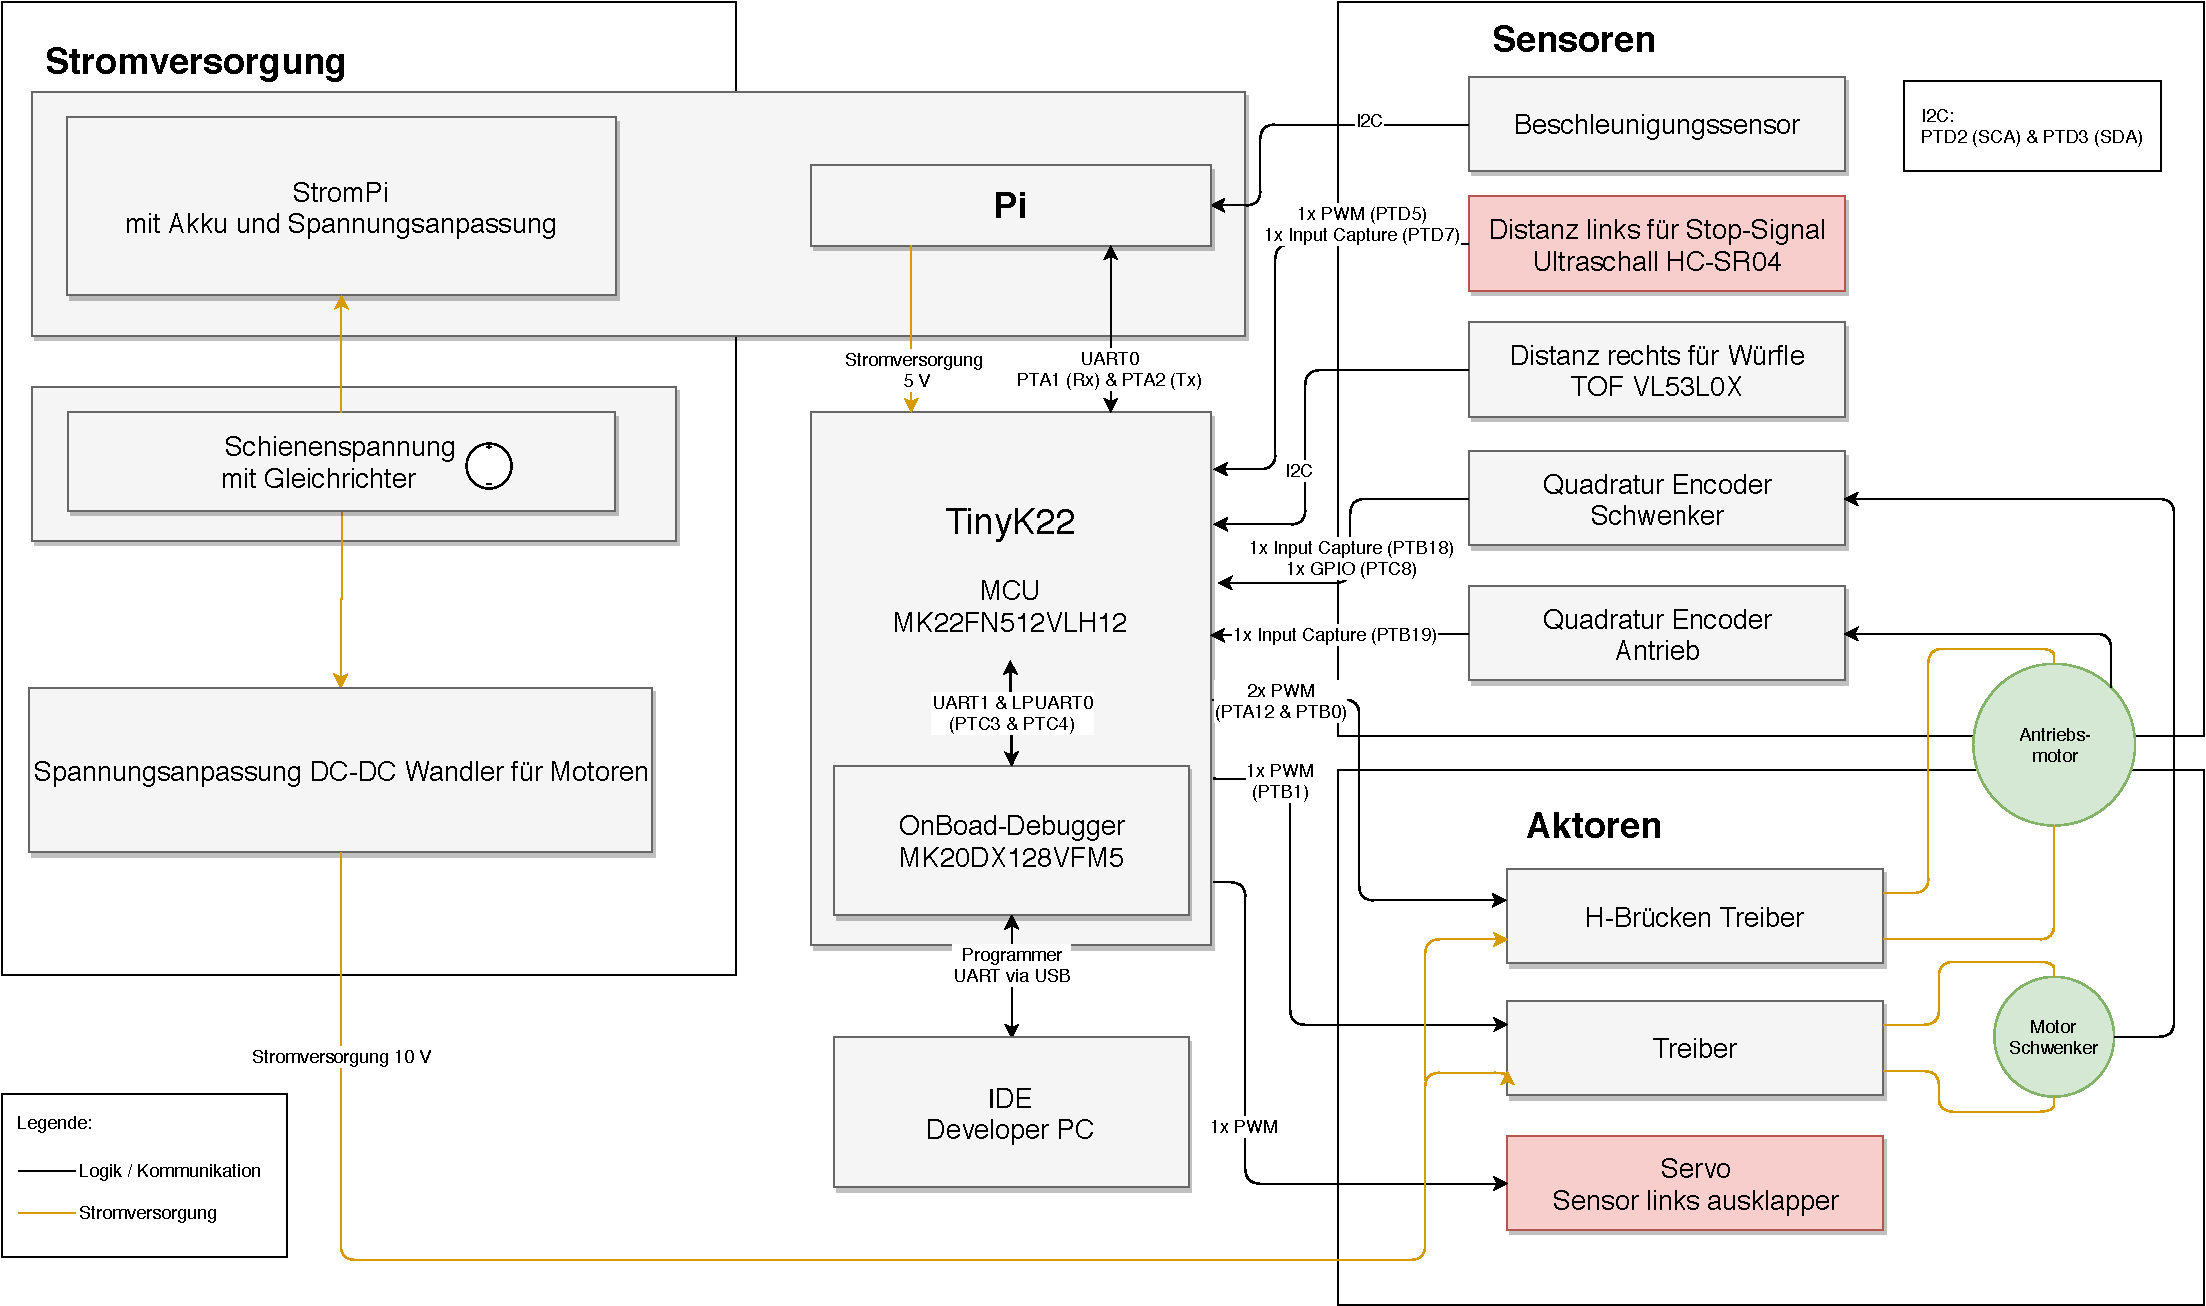
\includegraphics[width=1.0\textwidth]{../../images/et/KomponentenDiagramm_ET.pdf}
        \caption {Komponentendiagramm Elektronik}
        \label{fig:et_komponenten}
    \end{figure}

    Alle Verbindungen mit dem Tiny werden über Stecker auf einem PCB \footnote{PCB: Printed Circuit Board - Leiterplatte} verbunden. (siehe Abbildung \ref{fig:et_pcb}) Dies ermöglicht einen flexiblen modularen Aufbau. Auch die Gleichrichtung der Versorgungsspannung der Schienen erfolgt direkt auf dem PCB, sowie die nötigen Pegelwandlungen zwischen 3.3 V und 5 V der verschiedenen Komponenten.\\

    \begin{figure}[H]
        \centering
        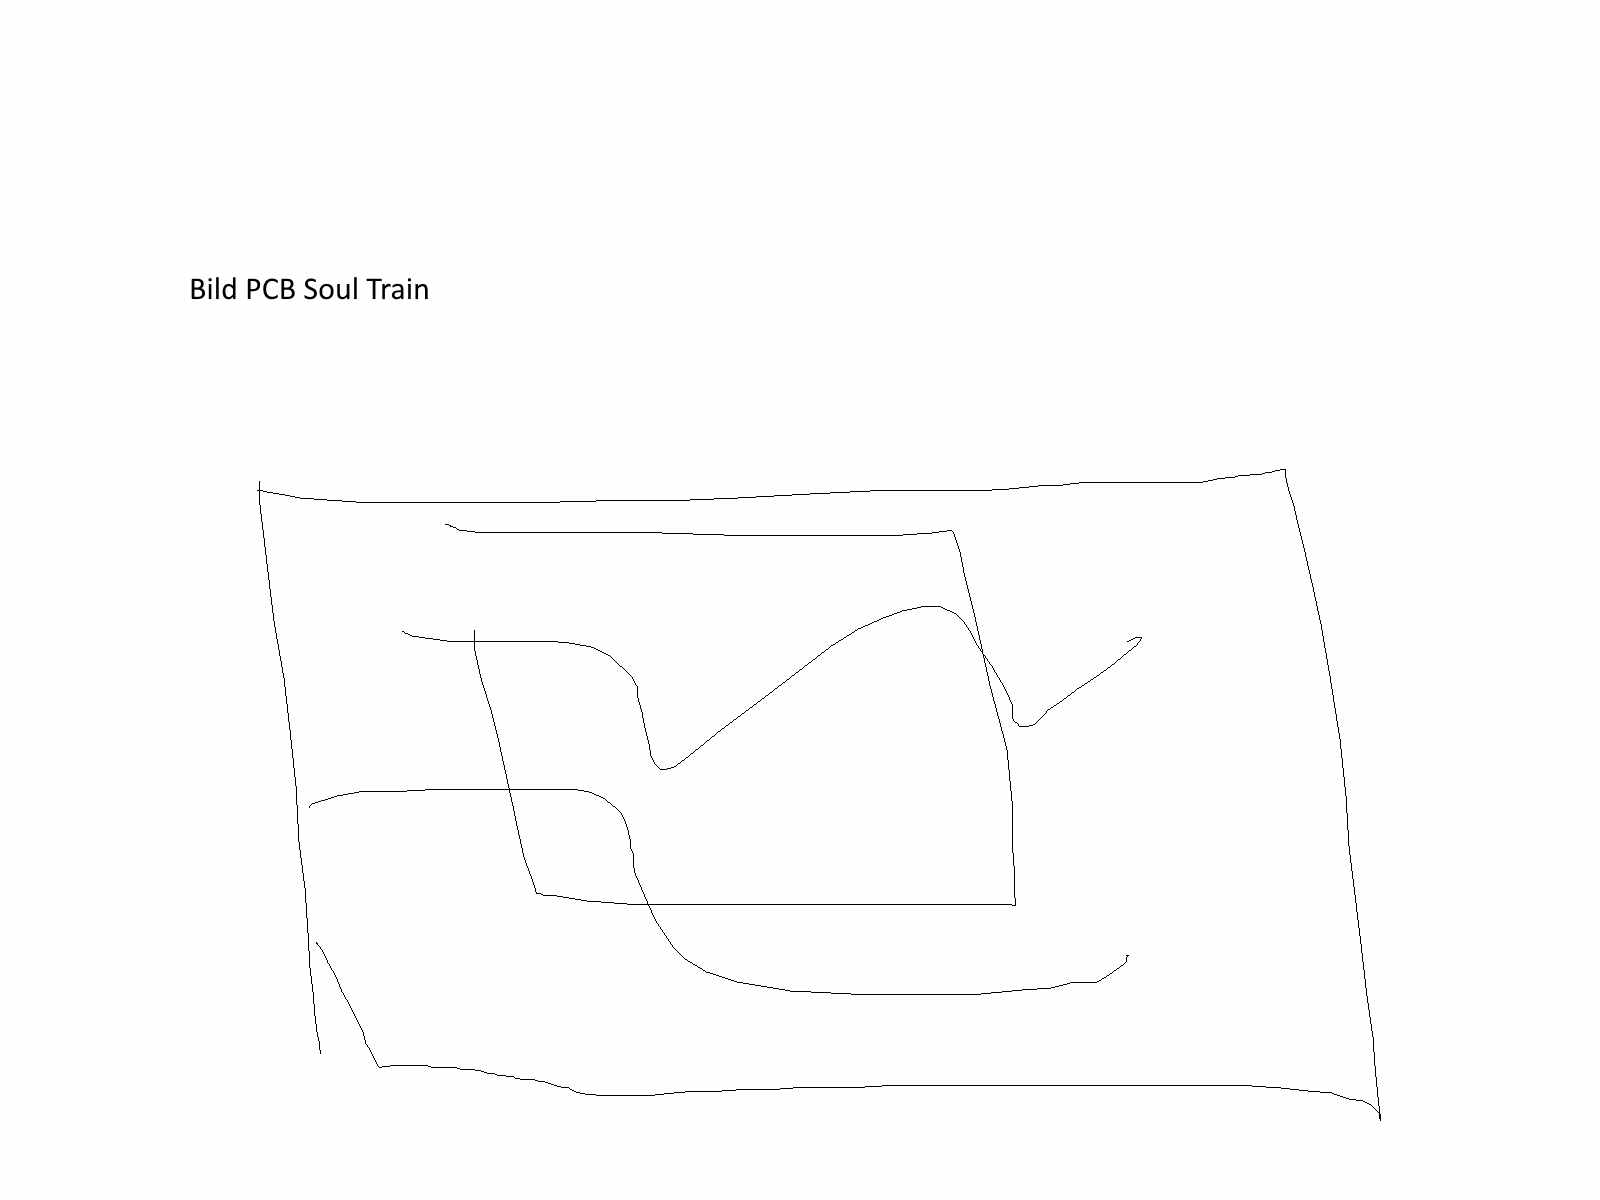
\includegraphics[width=0.7\textwidth]{../../images/et/et_pcb.jpg}
        \caption {PCB mit TinyK22}
        \label{fig:et_pcb}
    \end{figure}

    \subsubsection{Anordnung auf dem Zug} \label{et_anordnung}
    In Abbildung \ref{fig:et_anordnung} sind die Montierten Elektronik Komponenten ersichtlich. Die Komponenten wurden mit Schraub oder Klettverbindungen befestigt.\\

    \begin{figure}[H]
        \centering
        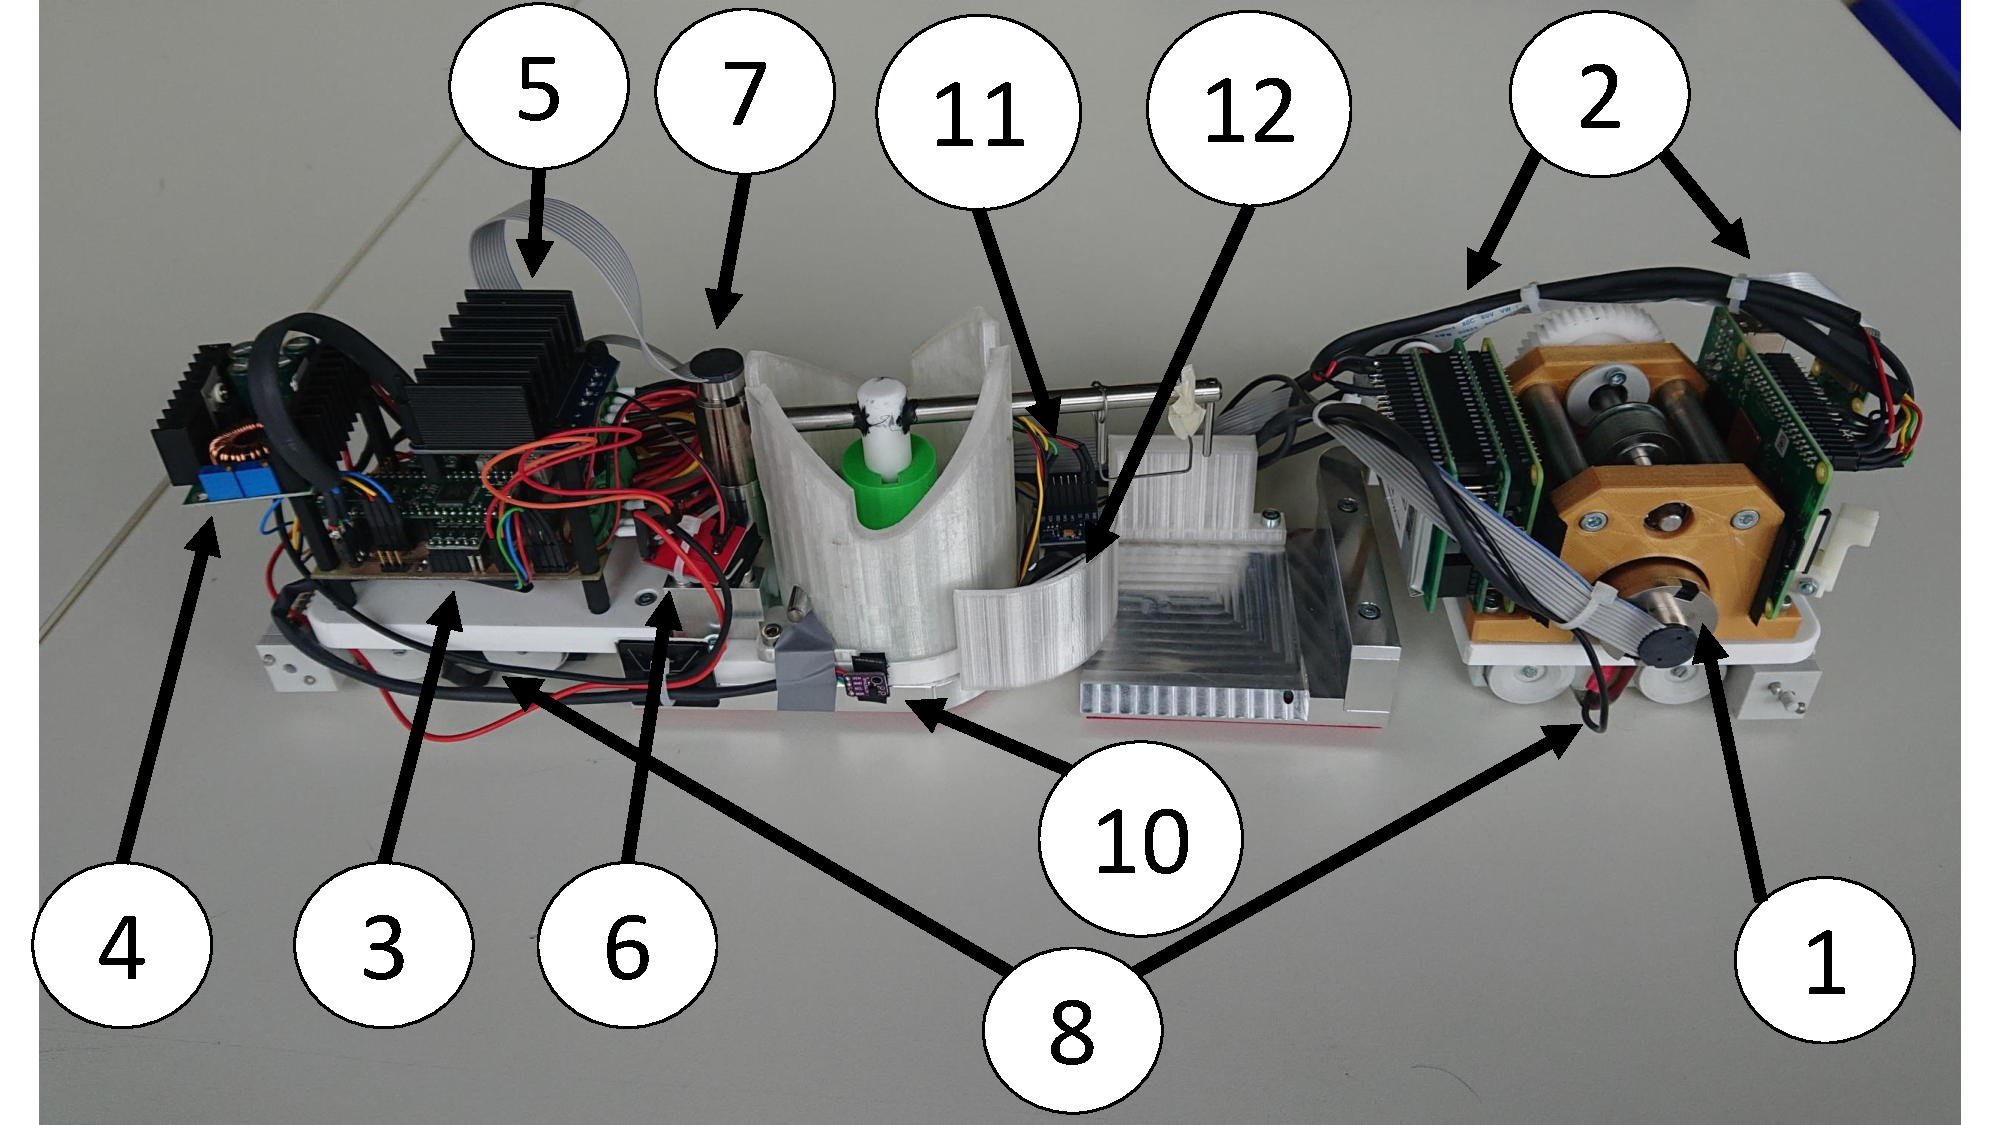
\includegraphics[width=1.0\textwidth]{../../images/et/et_anordnung_zug.pdf}
        \caption {Soul Train mit Elektronik}
        \label{fig:et_anordnung}
    \end{figure}

    An der Front des Zuges, an der Antriebseinheit mit Antriebsmotor [1], sind die beiden Raspberry Pi's [2] befestigt. Hinten auf dem Zug befindet sich das PCB [3] mit dem DC-DC Wandler [4] und den beiden Motorentreiber (Treiber [5] für den Antriebsmotor [1], Treiber [6] für den Schwenkermotor [7]). Direkt hinter der Schwenkervorrichtung ist der Motor für den Schwenker [7] befestigt. Jeweils zwischen den Räder befindet sich auf jeder Seite ein Schleifkontakt für die Stromabnahme von den Schienen [8]. Diese werden beide nach hinten geführt und auf das PCB [3] verbunden. Direkt unter dem Schwenkerarm ist der TOF-Sensor [10] für die Würfelerkennung montiert. Vor dem Schwenker befinden sich der Beschleunigungssensor [11] und der Buzzer [12]. Diese sind direkt mit dem Raspberry Pi verbunden und werden auch von dort angesteuert und ausgelesen.\\
     Alle Verbindungen sind mit Kabel auf der Rückseite des Zuges durchgeführt und befestigt. (siehe Abbildung \ref{fig:et_kabel})\\

    \begin{figure}[H]
        \centering
        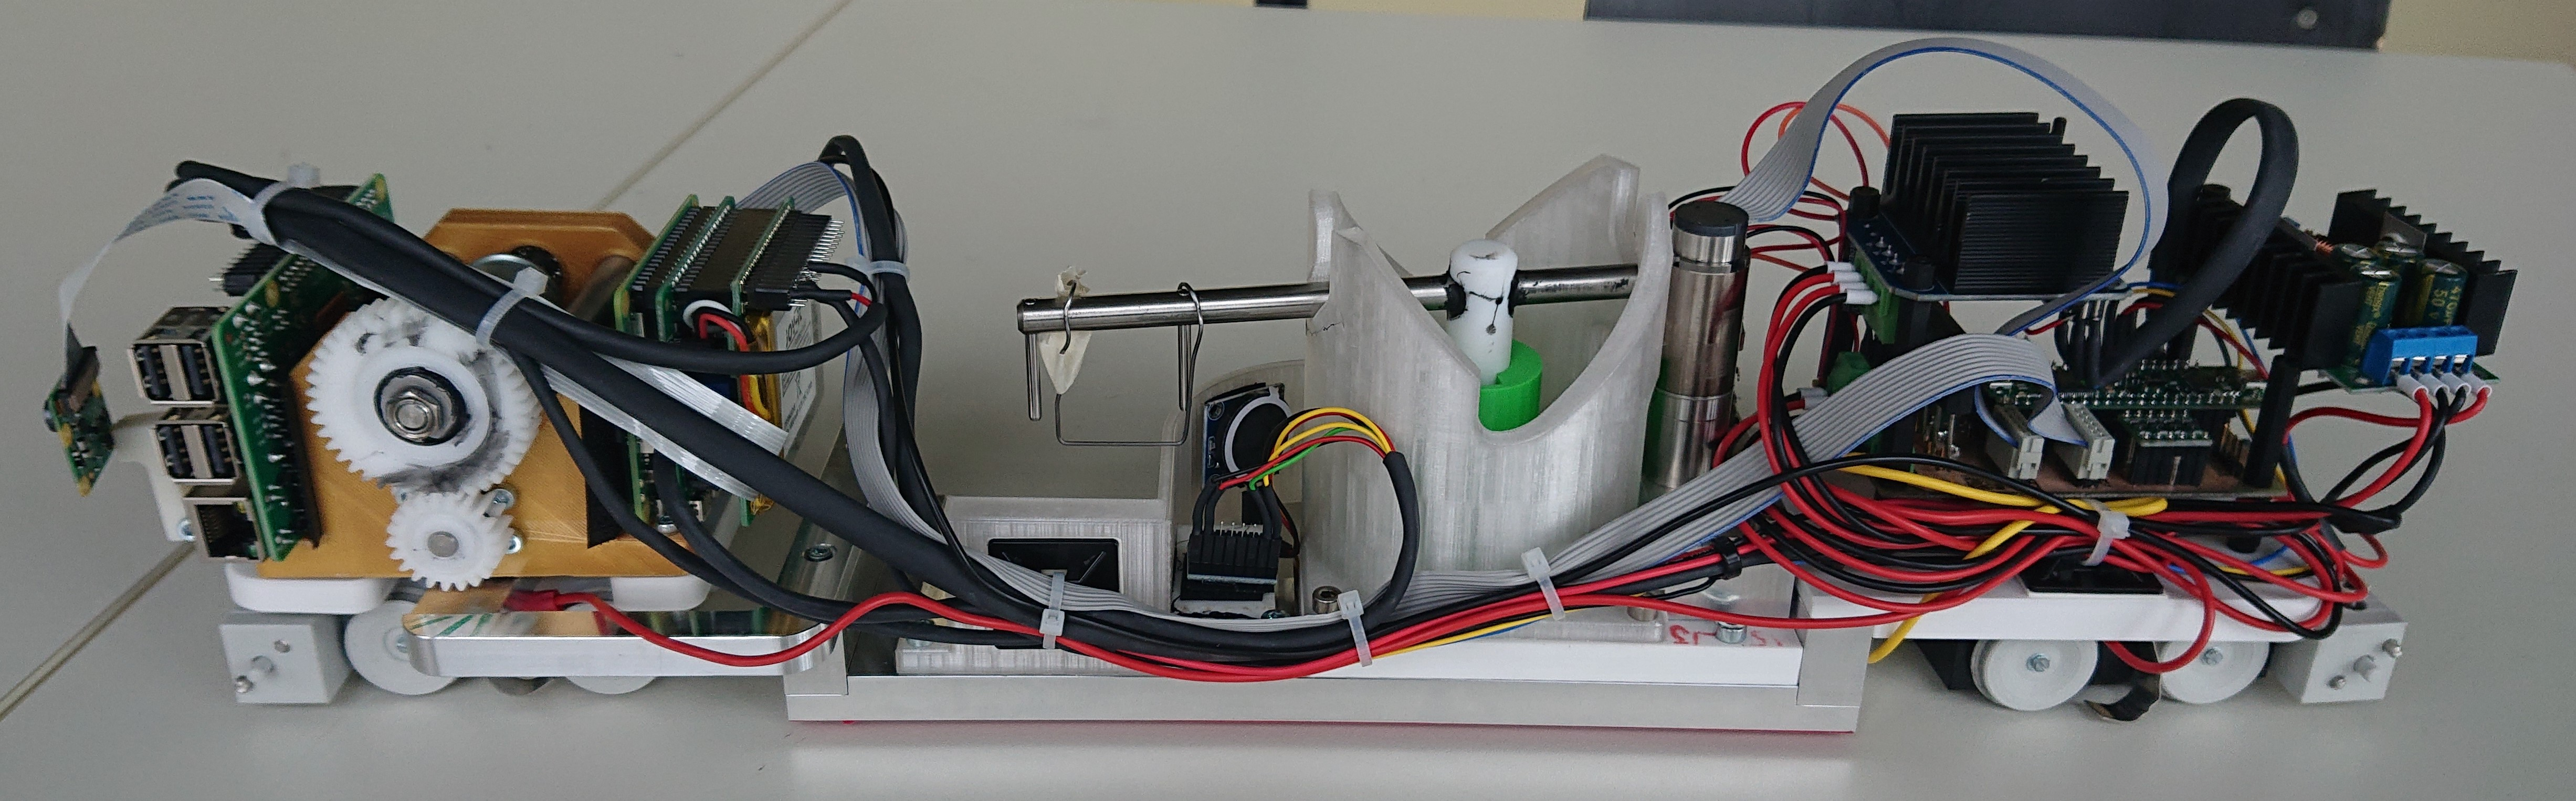
\includegraphics[width=1.0\textwidth]{../../images/et/et_kabel.jpg}
        \caption {Kabelverbindungen Rückseite}
        \label{fig:et_kabel}
    \end{figure}

    \subsection{Elektronik Komponenten} \label{et_Komponenten}
    In diesem Kapitel werden die einzelnen Komponenten beschreiben, die für die Steuerung des Soul Train verwendet werden. Dies beinhaltet alle Sensoren und Aktoren, die mit den Mikrocontroller TinyK22 verbunden sind.

    \subsubsection{Sensoren} \label{et_sensoren}
    Mit diversen Sensoren sollen folgende Daten aufgenommen werden.
    \begin{itemize}
        \item Geschwindigkeit
        \item Position
        \item Distanz rechts (Erkennung Würfel)
        \item zurückgelegter Winkel des Schwenkers
    \end{itemize}

    \textbf{Geschwindigkeit}\\
    Die Geschwindigkeit wird über den Quadratur Encoder am Antriebsmotor aufgenommen.\\
    Der Quadratur Encoder MR, Typ L gibt $1024$ Impulse pro Umdrehung. Der Verlauf eines Impulses ist in Abbildung \ref{fig:et_encoder} dargestellt. Der Encoder stellt drei Kanäle zur Verfügung. Über die Kanäle $A$ und $B$ kann einzeln die Geschwindigkeit bestimmt werden. Durch Auswerten der Phasenverschiebung der beiden Kanäle (''$A$ eilt $B$ vor'' oder ''$A$ eilt $B$ nach'') kann zusätzlich noch die Drehrichtung bestimmt werden. Der Kanal $I$ ist mit Kanal $A$ und $B$ synchronisiert und kann ebenfalls zur Bestimmung der Geschwindigkeit dienen.\\
    Für die Bestimmung der Geschwindigkeit kann die Dauer zwischen zwei Impulsen gemessen werden, oder es können die Anzahl Impulse in einer bestimmten Zeit gezählt werden. Für dieses Projekt werden die Anzahl Impulse in einer genau definierten Zeit gemessen. Dazu wird bei jedem Impuls ein Zähler inkrementiert und immer nach 10 ms ausgelesen und wieder zurückgesetzt. So kann immer über die letzten 10ms die Durchschnittsgeschwindigkeit bestimmt werden.\\

    \begin{wrapfigure}{r}{0.4\textwidth}
        \centering
        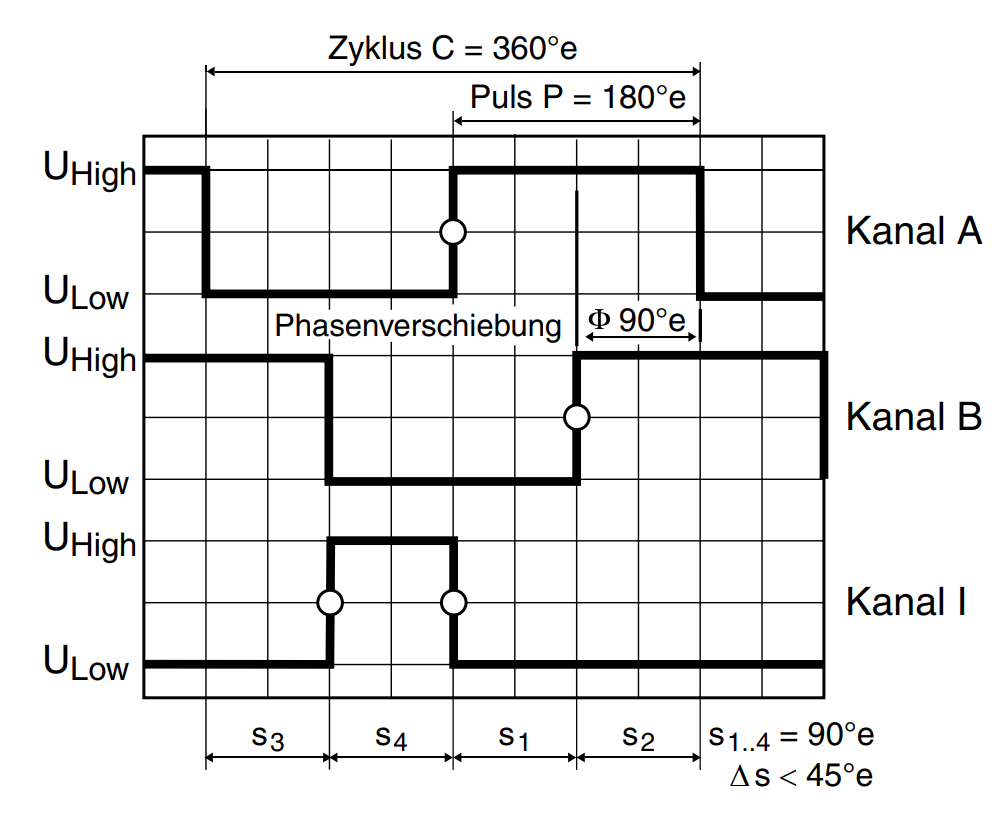
\includegraphics[width=0.4\textwidth]{../../images/et/Encoder_MR.png}
        \caption {Signalverlauf Encoder\\ (www.maxonmotor.ch)}
        \label{fig:et_encoder}
    \end{wrapfigure}

    Die Geschwindigkeit des Zuges ($v_{Zug}$) kann somit aus der Anzahl Impulsen ($Anz_{I}$)mittels der Mechanischen Übersetzung und der Grösse der Räder berechnet werden.
    \begin{equation} \label{eq:et_v_zug}
        v_{Zug}(Anz_{I}) = \frac{2 \cdot \pi \cdot Anz_{Impulse}}{\Delta T \cdot I_{Umdrehung} \cdot U}
    \end{equation}
    $r_r:$ Raddradius  $=13mm$\\
    $\Delta T:$  Messperiode  $=10ms$\\
    $I_{Umdrehung}:$  Impulse pro Umdrehung  $=1024$\\
    $U$  Mechanische Übersetzung  $=2$\\

    \textbf{Position}\\
    Durch das Zählen aller Impulse ab dem Start, kann die absolut zurückgelegte Distanz bestimmt werden. Diese Informationen wurde in der Umsetzung jedoch nicht benötigt und wurde somit auch nicht implementiert. Deshalb wird dies hier nicht weiter erläutert.

    
    \textbf{Distanz rechts (Erkennung Würfel) }\\
    Gemäss der Aufgabenstellung befindet sich der Würfel in einem Abstand von $8\pm1cm$ von der Gleismitte. Somit muss der Distanzsensor Distanzen zwischen ca. $20mm$ und $80mm$ erkennen können. Der exakte Wert der Distanz ist dabei nicht entscheidend, da nur ein bestimmter Schwellwert erkannt werden muss. Die Distanz zum Würfel wird mit einem TOF Sensor \footnote{TOF: Timo-Of-Flight} VL53L0X ermittelt. \\
    Dieser Schwellwert wird Messtechnisch ermittelt. Der Würfel wird an der vorgegebenen Position vor dem Sensor platziert (siehe Abbildung \ref{fig:et_tof_messung}) und der Wert ausgelesen. Dieser Wert kann dann in der Software festgelegt werden um zu entscheiden ob der Würfel erkannt wurde oder nicht. Der Wert des Sensors wird nicht in eine exakte Distanz umgerechnet, es wird direkt mit den rohen Sensorwerten der Schwellwert bestimmt. Mit der beschrieben Messung konnten mit dem Schwellwert $10000$ die zuverlässigsten Resultate erzielt werden.\\
    Der genaue Ablauf der Messung und Entscheidung der Software auf dem Tiny ist in Kapitel \ref{et_software_tiny_cube} beschreiben.\\

    \begin{figure}[H]
        \centering
        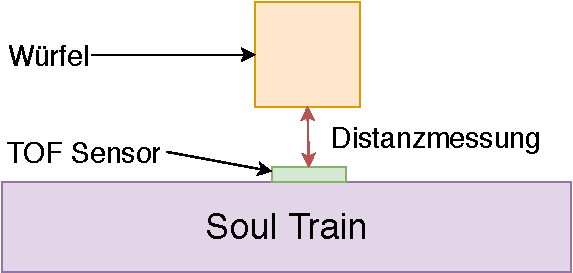
\includegraphics[width=0.6\textwidth]{../../images/et/et_tof_messung.pdf}
        \caption {Distanzmessung mit TOF Sensor}
        \label{fig:et_tof_messung}
    \end{figure}

    \textbf{Schwenkerwinkel}\\
    Um der Zurückgelegte Winkel des Schwenkers zu ermitteln ist auch auf dem Motor des Schwenkers ein Quadratur Encoder befestigt. Dieser Verhält sich vom Prinzip identisch wie der Encoder auf dem Antriebsmotor. Um den zurückgelegten Winkel zu ermitteln werden die Anzahl Impulse des Encoders gezählt. Der Motor muss den Schwenker drehen bis ein bestimmter Zielwert der Impulse erreicht ist. Dieser Zielwert wird mit der Mechanik messtechnisch ermittelt idem der Schwenker von Hand von der Start- bis zur Zielposition bewegt wird. (siehe Abbildung \ref{fig:et_schwenker_messung}) Die dabei gemessene Anzahlt Impulsen über die ganze Bewegung entspricht dem Zielwert.\\
    Diese Messung ergabe $5435$ Impulse für den nötigen Winkel.

    \begin{figure}[H]
        \centering
        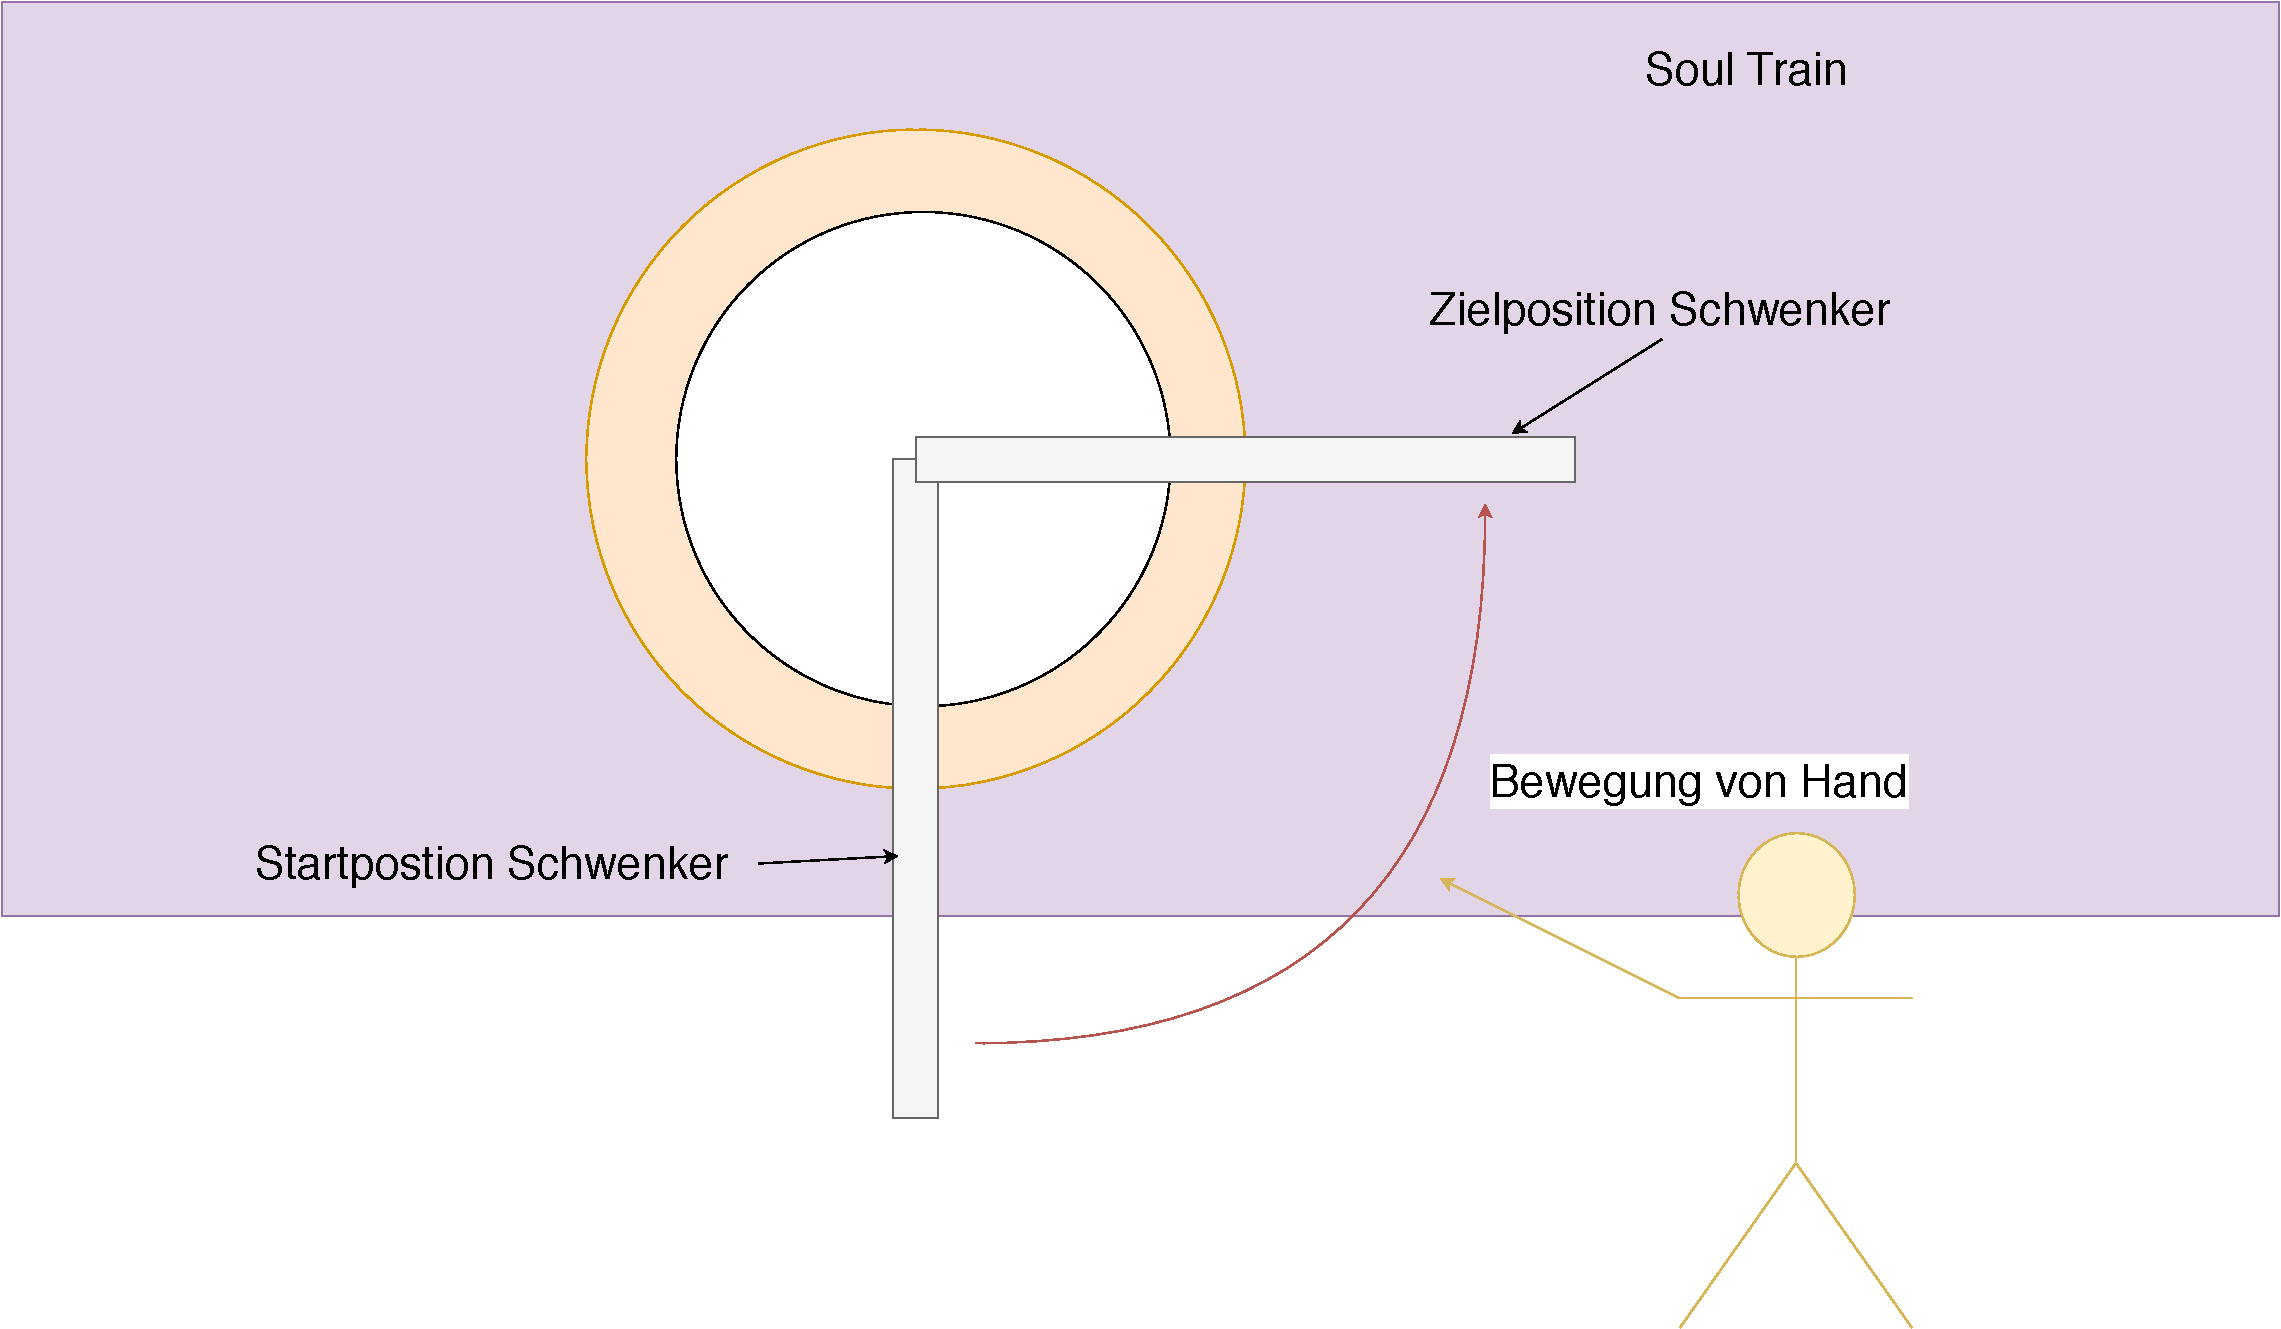
\includegraphics[width=0.9\textwidth]{../../images/et/et_schwenker_messung.pdf}
        \caption {Winkelmessung Schwenker}
        \label{fig:et_schwenker_messung}
    \end{figure}

    \subsubsection{Aktoren} \label{et_aktoren}
    Die Aktoren stellen die Schnittstelle zur Mechanik dar. Diese sollen alle nötigen mechanischen Bewegungen auf Befehl des Mikrocontrollers ausführen.\\

    \textbf{H-Brücken Treiber für Antriebsmotor}\\
    Um den Antriebsmotor anzusteuern, wird ein H-Brückentreiber verwendet. Damit kann der Motor durch ein PWM Signal in der Geschwindigkeit fast beliebig eingestellt werden. Über die wahlweise Ansteuerung einer der beiden Eingänge der H-Brücke wird die Richtung bestimmt.\\
    Es wird ein Arduion IBT\_2 DC-Motoren Treiber mit einem BTS7960 eingesetzt. Dieses Bauteil kann Motoren mit einem Strom von bis zu 43A versorgen. \\

    \textbf{Antriebsmotor}\\
    Als Antriebsmotor dient ein Maxon DCX 32 L. Dieser kann eine Leistung von bis zu 70 Watt umsetzen. \cite{MaxonDCX32L} Dies ist bei einer Versorgungsspannung von 24V spezifiziert. Da aber nicht die maximale Drehzahl benötigt wird, kann auch eine entsprechend tiefere Spannung angelegt werden. Die Drehzahlkonstante des Motors ist $350 \frac{min^{-1}}{V}$. Für die angestrebte Drehzahl von $5200min^{-1}$ ergibt sich eine Spannung von $$\frac{5200min^{-1}}{350 \frac{min^{-1}}{V}} =14.8V$$ Somit muss der Antriebsmotor mit einer Spannung von $14.8V$ versorgt werden.\\\textbf{\color{red}{TODO:korrekt verwendete Spannung einsetzen!}}

    \textbf{Motortreiber für Schwenker-Motor}\\
    Da die Richtung immer dieselbe ist reicht für den Schwenker ein normaler DC-Motoren Treiber. Um eine sanfte Beschleunigung und Bremsung der Konstruktion zu ermöglichen, wird auch der Schwenker-Motor mit einem PWM angesteuert. Als Treiber wird ein Board mit einem L298N verwendet.\\

    \textbf{Schwenker-Motor}\\
    Für den Schwenker wird ein Maxon DCX 19 S verwendet. Um die Position des Schwenkers zu bestimmen, ist auch an diesem Motor ein Encoder befestigt. Die verwendung deses Encoders ist in Kaptitel \ref{et_sensoren} beschrieben. \cite{MaxonDCX19S}\\

    \end{document}
